\documentclass{article}%
\usepackage{amsmath}
\usepackage{amsfonts}
\usepackage{amssymb}
\usepackage{listings}
\usepackage{graphicx}
\usepackage{tikz}
\usepackage{hyperref}%
\usepackage[a4paper,includeheadfoot,margin=0.5in]{geometry}
\setcounter{MaxMatrixCols}{30}
%TCIDATA{OutputFilter=late$x2$.dll}
%TCIDATA{Version=5.00.0.2552}
%TCIDATA{CSTFile=40 LaTeX article.cst}
%TCIDATA{Created=Thursday, August 21, 2008 14:03:59}
%TCIDATA{LastRevised=Wednesday, October 01, 2014 12:46:33}
%TCIDATA{<META NAME="GraphicsSave" CONTENT="32">}
%TCIDATA{<META NAME="SaveForMode" CONTENT="1">}
%TCIDATA{<META NAME="DocumentShell" CONTENT="Standard LaTeX\Blank - Standard LaTeX Article">}
%TCIDATA{Language=American English}
\newtheorem{theorem}{Theorem}
\newtheorem{acknowledgement}[theorem]{Acknowledgement}
\newtheorem{algorithm}[theorem]{Algorithm}
\newtheorem{axiom}[theorem]{Axiom}
\newtheorem{case}[theorem]{Case}
\newtheorem{claim}[theorem]{Claim}
\newtheorem{conclusion}[theorem]{Conclusion}
\newtheorem{condition}[theorem]{Condition}
\newtheorem{conjecture}[theorem]{Conjecture}
\newtheorem{corollary}[theorem]{Corollary}
\newtheorem{criterion}[theorem]{Criterion}
\newtheorem{definition}[theorem]{Definition}
\newtheorem{example}[theorem]{Example}
\newtheorem{exercise}[theorem]{Exercise}
\newtheorem{lemma}[theorem]{Lemma}
\newtheorem{notation}[theorem]{Notation}
\newtheorem{problem}[theorem]{Problem}
\newtheorem{proposition}[theorem]{Proposition}
\newtheorem{remark}[theorem]{Remark}
\newtheorem{solution}[theorem]{Solution}
\newtheorem{summary}[theorem]{Summary}
\newenvironment{proof}[1][Proof]{\noindent\textbf{#1.} }{\ \rule{0.5em}{0.5em}}

\usepackage{fancyhdr}
\setlength\headheight{26pt}
\pagestyle{fancy}
\lhead{{\footnotesize Assignment 14}}
\rhead{{\footnotesize Christopher Chapline}}
\begin{document}

\section*{Problem 1}
\subsection*{Part 1}

This is the language consisting of a string starting with either an $a$ or $b$,
followed by zero or more $a$'s, ending in either an $a$ or $b$.

\subsection*{Part 2}
\begin{center}
    \begin{tikzpicture}[scale=0.2]
        \tikzstyle{every node}+=[inner sep=0pt]
        \draw [black] (17.7,-30.6) circle (3);
        \draw (17.7,-30.6) node {$S$};
        \draw [black] (32.5,-30.6) circle (3);
        \draw (32.5,-30.6) node {$A$};
        \draw [black] (46,-30.6) circle (3);
        \draw (46,-30.6) node {$A_1$};
        \draw [black] (46,-30.6) circle (2.4);
        \draw [black] (20.089,-28.803) arc (118.71395:61.28605:10.43);
        \fill [black] (30.11,-28.8) -- (29.65,-27.98) -- (29.17,-28.86);
        \draw (25.1,-27.02) node [above] {$a$};
        \draw [black] (31.177,-27.92) arc (234:-54:2.25);
        \draw (32.5,-23.35) node [above] {$a$};
        \fill [black] (33.82,-27.92) -- (34.7,-27.57) -- (33.89,-26.98);
        \draw [black] (34.767,-28.657) arc (120.78176:59.21824:8.76);
        \fill [black] (43.73,-28.66) -- (43.3,-27.82) -- (42.79,-28.68);
        \draw (39.25,-26.92) node [above] {$a$};
        \draw [black] (30.042,-32.304) arc (-63.12886:-116.87114:10.934);
        \fill [black] (30.04,-32.3) -- (29.1,-32.22) -- (29.55,-33.11);
        \draw (25.1,-33.98) node [below] {$b$};
        \draw [black] (43.613,-32.396) arc (-62.22669:-117.77331:9.363);
        \fill [black] (43.61,-32.4) -- (42.67,-32.33) -- (43.14,-33.21);
        \draw (39.25,-33.97) node [below] {$b$};
        \draw [black] (9.2,-30.6) -- (14.7,-30.6);
        \draw (8.7,-30.6) node [left] {$start$};
        \fill [black] (14.7,-30.6) -- (13.9,-30.1) -- (13.9,-31.1);
    \end{tikzpicture}
\end{center}

\section*{Problem 2}
\begin{center}
    \begin{tikzpicture}[scale=0.2]
        \tikzstyle{every node}+=[inner sep=0pt]
        \draw [black] (17.7,-30.6) circle (3);
        \draw (17.7,-30.6) node {$S$};
        \draw [black] (32.5,-30.6) circle (3);
        \draw (32.5,-30.6) node {$A$};
        \draw [black] (46,-30.6) circle (3);
        \draw (46,-30.6) node {$A_1$};
        \draw [black] (46,-30.6) circle (2.4);
        \draw [black] (20.089,-28.803) arc (118.71395:61.28605:10.43);
        \fill [black] (30.11,-28.8) -- (29.65,-27.98) -- (29.17,-28.86);
        \draw (25.1,-27.02) node [above] {$a$};
        \draw [black] (31.177,-27.92) arc (234:-54:2.25);
        \draw (32.5,-23.35) node [above] {$a$};
        \fill [black] (33.82,-27.92) -- (34.7,-27.57) -- (33.89,-26.98);
        \draw [black] (34.767,-28.657) arc (120.78176:59.21824:8.76);
        \fill [black] (43.73,-28.66) -- (43.3,-27.82) -- (42.79,-28.68);
        \draw (39.25,-26.92) node [above] {$a$};
        \draw [black] (30.042,-32.304) arc (-63.12886:-116.87114:10.934);
        \fill [black] (30.04,-32.3) -- (29.1,-32.22) -- (29.55,-33.11);
        \draw (25.1,-33.98) node [below] {$b$};
        \draw [black] (43.613,-32.396) arc (-62.22669:-117.77331:9.363);
        \fill [black] (43.61,-32.4) -- (42.67,-32.33) -- (43.14,-33.21);
        \draw (39.25,-33.97) node [below] {$b$};
        \draw [black] (9.2,-30.6) -- (14.7,-30.6);
        \draw (8.7,-30.6) node [left] {$start$};
        \fill [black] (14.7,-30.6) -- (13.9,-30.1) -- (13.9,-31.1);
        \draw [black] (44.284,-33.055) arc (-40.23426:-139.76574:16.287);
        \fill [black] (19.42,-33.06) -- (19.55,-33.99) -- (20.31,-33.34);
        \draw (31.85,-39.32) node [below] {$\epsilon$};
    \end{tikzpicture}
\end{center}

\section*{Problem 3}

Determinism is not important because any non-deterministic automaton can be
converted into a deterministic automaton. Similarly, any incomplete automaton can be
converted into a complete automaton with the addition of a hell state.


\end{document}
